\documentclass[10pt]{article}
\usepackage{graphicx}
\begin{document}
\title{Introduction to Kernel Modules()}
\author{Paul D. Camarata}

\maketitle
\pagebreak
\begin{abstract}
"I do not fear computers. I fear lack of them."
-Isaac Asimov
\end{abstract}

\section{Introduction}
The purpose of this programming project was to gain a better understanding of kernel modules.  It is broken apart into four sections, each of which was a different lesson on different aspects of how an operating system sees and uses kernel modules.

\section{Part I: Kernel Modules Overview}
Part I is dedicated to listing and compiling of kernel modules.  The images included are here to reference the work that was done locally.

Figure 12 is a reference to running the 'lsmod' command.  I have shortened the output, but this command showed that there are many modules currently running on my system.

\begin{figure}[!h]
\centering
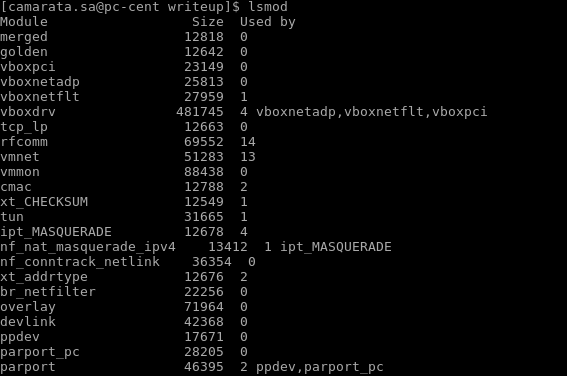
\includegraphics[scale=0.5]{./images/ss1.png}
\caption{lsmod}
\label{fig:Code}
\end{figure}

Figure 2 is a reference to the 'make' command.  Upon further examination of the make file, it looks like it is grabbing my currently loaded kernel via 'uname -r' and leveraging that as conditional input to create the binary that will be loaded later.

\begin{figure}[!h]
\centering
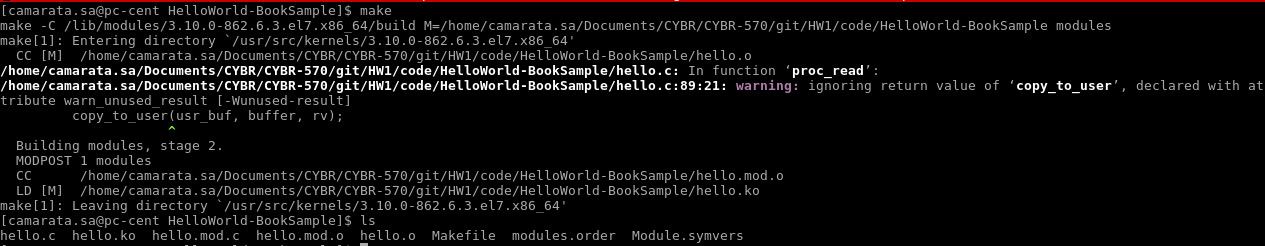
\includegraphics[scale=0.5]{./images/ss2.png}
\caption{make}
\label{fig:Code}
\end{figure}

\section{Part II: Loading and Removing Kernel Modules}
If the title of this section doesn't give it away, then I'm not sure how else I can explain this section.  Here we are taking the resulting file(s) from the previous 'make' execution, specifically the '.ko' file and loading it as a kernel module via the 'insmod \{module\_file\_name\}' command.

\begin{figure}[!h]
\centering
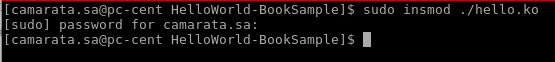
\includegraphics[scale=0.5]{./images/ss3.png}
\caption{insmod}
\label{fig:Code}
\end{figure}

Executing this command adds a log in the 'dmesg' buffer which we examine in Figure 4.

\begin{figure}[!h]
\centering
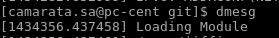
\includegraphics[scale=0.5]{./images/ss4.png}
\caption{dmesg - add}
\label{fig:Code}
\end{figure}

We then remove the module using 'rmmod \{module\_name\}' command...

\begin{figure}[!h]
\centering
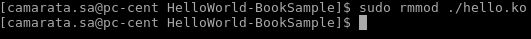
\includegraphics[scale=0.5]{./images/ss5.png}
\caption{rmmod}
\label{fig:Code}
\end{figure}

And then we examine 'dmesg' a final time to view the exit message.

\begin{figure}[!h]
\centering
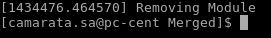
\includegraphics[scale=0.5]{./images/ss6.png}
\caption{dmesg - remove}
\label{fig:Code}
\end{figure}

\pagebreak

From here we start to write some of our own code.  All code from this assignment is included here as an appendix as well as delivered as an additional document for the instructor's convenience.  As a side note, all deliverables for this assignment are also available via https://github.com/paulcamarata/CYBR-570.  Rather than step through every component that needed to be done to complete this portion, I will include the parts that I believe are key and let the included code speak for how this was accomplished.

The initial goal was to print the GOLDEN\_RATIO\_PRIME as part of the module initialization.  Figure 7 displays the results when executing this.  The one thing to note is that this value appears to be different than what was expected.  I worked on this partnered with a couple of other students and this 'delta' had me dig a little bit deeper.  I figured the discrepancy existed because I was using a different operating system then my fellow students, but I wanted to understand why my value was so much different, considering this value seemed like it should have been a constant to me.  Sure enough, when I dug into the hash.h header file, there were two constants declared, GOLDEN\_Ratio\_32 and GOLDEN\_RATIO\_64.  When I translated the value of them from hex to binary, the numbers matched up.  Also, since I was leveraging a 64 bit kernel, I was defaulting to a value that was different from my classmates.  I also tried this on a 64 bit Ubuntu machine, and the value was different yet again.  I did not do further research to understand why the 64 bit value is different, even among other seemingly similar operating systems.

\begin{figure}[!h]
\centering
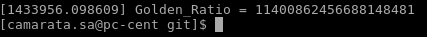
\includegraphics[scale=0.5]{./images/ss7.png}
\caption{GOLDEN\_RATIO}
\label{fig:Code}
\end{figure}

The last portion of part 2 was to have the 'gcd' function return the greatest common denominator of 3,300 and 24.  The results of this are below in Figure 8.

\begin{figure}[!h]
\centering
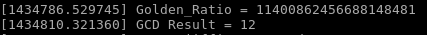
\includegraphics[scale=0.5]{./images/ss8.png}
\caption{GCD}
\label{fig:Code}
\end{figure}

\pagebreak
\section{Part III}
Part 3 was all about learning how to get something that is dynamically read when called in the proc virtual file system (VFS).  This VFS is used to convey all sorts of information that is generally made available by the kernel.  The setup of this portion was not part of the deliverable, but it was instrumental for setting up Part 4.

\section{Part IV}
Part 4 is the real meat and potatoes of the assignment.  The goal here was to implement two different proc entries that would yield differing results when queried.  The first was to create a VFS entry for /proc/jiffies.  The results of this are included in Figure 9.

\begin{figure}[!h]
\centering
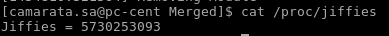
\includegraphics[scale=0.5]{./images/ss9.png}
\caption{Jiffies}
\label{fig:Code}
\end{figure}

The second deliverable for Part 4 was to create a VFS entry for /proc/seconds that would report the amount of time since the module had been loaded in seconds.  The results of this command can be seen in Figure 10.

\begin{figure}[!h]
\centering
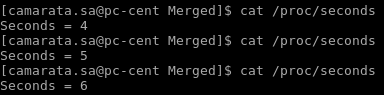
\includegraphics[scale=0.5]{./images/ss10.png}
\caption{Seconds}
\label{fig:Code}
\end{figure}

It is important to note that in order to accomplish this, I had to create a global variable that the kernel can leverage to pass the value of jiffies on initialization to the application.  Reading implied that doing it this way is bad.

\section{Conclusion}
In conclusion, I think this was an interesting coding project.  I would definitely be curious about more practical examples of kernel modules, or a project that dives a bit deeper.  I feel like with the code that was provided as a template, this project was overly basic for what I think an engineer in a Master's program should be capable of doing.  To attempt to compensate this, I worked with a fellow classmate to try and get all of the components into one C file that is included in the appendix.  I also wrote this paper using LaTeX to try and learn something new.

\pagebreak
\section{Appendix A: Code}
\begin{verbatim}
#include <linux/init.h>
#include <linux/module.h>
#include <linux/kernel.h>
#include <linux/proc_fs.h>
#include <asm/uaccess.h>
#include <linux/hash.h>
#include <linux/gcd.h>

#define BUFFER_SIZE 128

#define PROC1_NAME "jiffies"
#define PROC2_NAME "seconds"
#define MESSAGE "Hello World\n"

long unsigned jiffies_var = 0;

/**
 * Function prototypes
 */
ssize_t read_jiffies(struct file *file, char *buf, size_t count, loff_t *pos);
ssize_t read_seconds(struct file *file, char *buf, size_t count, loff_t *pos);


static struct file_operations proc_ops_jiffies = {
        .owner = THIS_MODULE,
        .read = read_jiffies,
};

static struct file_operations proc_ops_seconds = {
        .owner = THIS_MODULE,
        .read = read_seconds,
};

/* This function is called when the module is loaded. */
int proc_init(void)
{

        // creates the /proc/golden entry
        // the following function call is a wrapper for
        // proc_create_data() passing NULL as the last argument
        proc_create(PROC1_NAME, 0, NULL, &proc_ops_jiffies);
        proc_create(PROC2_NAME, 0, NULL, &proc_ops_seconds);

        jiffies_var = jiffies;

        printk(KERN_INFO "Loading Module\n");
        printk(KERN_INFO "/proc/%s created\n", PROC1_NAME);
        printk(KERN_INFO "/proc/%s created\n", PROC2_NAME);
        printk(KERN_INFO "Jiffies = %lu\n", jiffies);
        printk(KERN_INFO "Golden_Ratio = %lu\n", GOLDEN_RATIO_PRIME);
	return 0;
}

/* This function is called when the module is removed. */
void proc_exit(void) {
        // removes the /proc/golden entry
        remove_proc_entry(PROC1_NAME, NULL);
        remove_proc_entry(PROC2_NAME, NULL);

        printk( KERN_INFO "GCD Result = %lu\n", gcd(3300,24));

        printk( KERN_INFO "/proc/%s removed\n", PROC1_NAME);
        printk( KERN_INFO "/proc/%s removed\n", PROC2_NAME);
        printk(KERN_INFO "Removing Module\n");

}

/**
 * This function is called each time the /proc/golden is read.
 * 
 * This function is called repeatedly until it returns 0, so
 * there must be logic that ensures it ultimately returns 0
 * once it has collected the data that is to go into the 
 * corresponding /proc file.
 *
 * params:
 *
 * file:
 * buf: buffer in user space
 * count:
 * pos:
 */
ssize_t read_jiffies(struct file *file, char __user *usr_buf, size_t count, loff_t *pos)
{
        int rv = 0;
        char buffer[BUFFER_SIZE];
        static int completed = 0;

        if (completed) {
                completed = 0;
                return 0;
        }

        completed = 1;

        rv = sprintf(buffer, "Jiffies = %lu\n", jiffies);

        // copies the contents of buffer to userspace usr_buf
        copy_to_user(usr_buf, buffer, rv);

        return rv;
}

ssize_t read_seconds(struct file *file, char __user *usr_buf, size_t count, loff_t *pos)
{
        int rv = 0;
        long unsigned time = 0;
        char buffer[BUFFER_SIZE];
        static int completed = 0;

        if (completed) {
                completed = 0;
                return 0;
        }

        completed = 1;
        time = jiffies/HZ - jiffies_var/HZ;
        rv = sprintf(buffer, "Seconds = %lu\n", time);

        // copies the contents of buffer to userspace usr_buf
        copy_to_user(usr_buf, buffer, rv);

        return rv;
}

/* Macros for registering module entry and exit points. */
module_init( proc_init );
module_exit( proc_exit );

MODULE_LICENSE("GPL");
MODULE_DESCRIPTION("CYBER-570 Assignment 1");
MODULE_AUTHOR("Paul Camarata");

\end{verbatim}

\end{document}
